\documentclass[11pt, a4paper, oneside, titlepage, headsepline]{book}

\usepackage{a4}
\usepackage{epsf}	% to import eps pictures
\usepackage{graphicx}	% Import graphics and figures
\usepackage{amsmath}	% Mathematical expressions
\usepackage{url}		% Urls are used
\usepackage{packages/apalike/apalike}	% To use the apalike bibliography style
\usepackage{glosstex}
\usepackage{setspace}	% set line spacing
\usepackage[german,english]{babel}

\usepackage[automark]{scrpage2}
\usepackage{blindtext}
\clearscrheadings
\rohead{\rightmark}
\lehead[]{}
\ofoot[]{}
\cfoot[\pagemark]{\pagemark}
\pagestyle{scrheadings}


\onehalfspacing

\setlength{\parindent}{0em}		% do not indent at the beginning of a paragraph
\setlength{\parskip}{11pt}		% Set distance between two paragraphs

% Begin the document
\begin{document}

% Set english as language
\selectlanguage{english}

% Document information
\author{Daniel Kuster}
\title{Infiltrating wireless networks and intrusion detection - A hybrid approach using neural networks}
\date{2006}

% Display roman page numbers
\frontmatter

% Create the first page
% The cover of the thesis 123

% So that no pagenumber is written
\begin{titlepage}

\begin{figure}[htb]
   \hspace{2mm}
   \begin{minipage}[c]{10.5cm}
    \LARGE \bf Fachhochschule Vorarlberg GmbH.
   \end{minipage}
   \hfill
   \begin{minipage}[c]{1.5cm}
    \setlength{\epsfxsize}{1cm}
    \epsfbox{graphics/Logo_fhv.eps}
	%
\includegraphics[height=1cm]{graphics/Logo_fhv}
	%
\includegraphics{graphics/Logo_fhv}
   \end{minipage}
   \hspace{2mm}
\end{figure}

\fbox{
  \parbox{0.94\textwidth}{
    %\vspace{2em}
	\vspace{4em}
    \centerline{Diplomarbeit im}
    \centerline{Fachhochschul-Diplomstudiengang}
    \centerline{iTec - Information and Communication Engineering}
    \vspace{4em}

    {\LARGE \centerline{\bf \em Infiltrating Wireless Networks}
			\centerline{\bf \em and Intrusion Detection}
           \centerline{\em A Hybrid Approach using Neural Networks}
           \centerline{\bf \em }}
    \vspace{9em}
    \centerline{ausgef\"uhrt von}
    \vspace{1em}
    \centerline{\bf Daniel Kuster}
	\vspace{1em}
%    \centerline{\bf H\"ammerlestrasse 11b, 6800 Feldkirch}
    \centerline{\bf 021 0109 009}
    \vspace{4em}
    \centerline{Dornbirn, im \bf August 2006}
    \vspace{4em}
    \centerline{\small Betreuer: \bf DI Patrick Ritschel}
    \vspace{2em}
  }
}
 
\end{titlepage}


\cfoot[\pagemark]{\pagemark}

% Create the rest of the document

% Set english as language
\selectlanguage{german}

\pagenumbering{roman}

\chapter*{Eidesstattliche Erkl\"arung}

Ich erkl\"are hiermit ehrenw\"ortlich, dass ich die vorliegende Arbeit selbstst\"andig angefertigt habe. Die aus fremden Quellen direkt oder indirekt \"ubernommenen Gedanken sind als solche kenntlich gemacht. Die Arbeit wurde bisher keiner anderen Pr\"ufungsbeh\"orde vorgelegt und auch noch nicht ver\"offentlicht. \vspace{3cm}

%\begin{center}

\begin{table}[htbp]
	\begin{center}
		\begin{tabular}{p{250pt}}
		\hline
			\vspace{0ex}
			\centerline{{\bf{Kuster Daniel}}, Feldkirch 20. August 2006}
		\end{tabular}
	\end{center}
\end{table}

\chapter*{Danksagung}

Zuerst m\"ochte ich meinen Eltern, {\bf Ingrid} und {\bf Helmut Kuster}, danken, die mir w\"ahrend des ganzen Studiums den notwendigen Freiraum zukommen lie"sen, den ich gebraucht habe. Sie haben nie versucht, mich von etwas anderem \"uberzeugen, sondern haben mich in all meinem Handeln best\"arkt. Ohne sie w\"are mir mein Studium an der FH Dornbirn, auch dank ihrer finanziellen Unterst\"utzung, verwehrt geblieben.

Ich m\"ochte meiner Freundin {\bf Elisabeth Bertsch} daf\"ur danken, dass sie mich in allem was ich tue unterst\"utzt. Sie ist eine wunderbare Zuh\"orerin. Sie bietet mir den Halt den ich ben\"otige, wenn ich Probleme habe oder bei meiner Arbeit ins Stocken gerate.

Zuguterletzt m\"ochte ich auch meinem Betreuer {\bf Patrick Ritschel} danken, der mir bei auftretenden Problemen und Fragen immer hilfreich zur Seite gestanden hat. Er hat mich stets beraten und Hilfestellungen geboten, wo sie notwendig waren. Ich m\"ochte ihm auch daf\"ur danken, dass er mir selbstst\"andiges Arbeiten erm\"oglicht hat, um meinen eigenen Ideen und Wegen nachgehen zu k\"onnen.

\chapter*{Zusammenfassung}

Diese Diplomarbeit zeigt die Machbarkeit und Implementierung eines Einbruchs-erkennungssystems f\"ur WLANs (WIDS), welches ein neurales Netzwerk (ANN) zur Erkennung von verschiedenen Attacken verwendet.

Nach der theoretischen Einf\"uhrung in die Themen WLAN und neurale Netzwerke, werden einige, im Internet frei verf\"ugbare Programme, die zum Mith\"oren von Netzwerkpaketen, zum Brechen der WEP Verschl\"usselung und zur Einbruchs-erkennung verwendet werden,  vorgestellt. Im letzten Teil werden Details, des zu implementierenden WIDS, beschrieben und Verbesserungsvorschl\"age diskutiert.

Das WIDS besteht aus vier Teilen:

Die erste Komponente, genannt {\em data gatherer}, holt sich Netzwerkpakete entweder aus einer Datei oder direkt von der Netzwerkkarte. Die zweite Komponente, {\em data processor}, enth\"alt das neurale Netzwerk, welches f\"ur das Lernen der Charakteristika von verschiedenen Attacken verantwortlich ist und einen Pr\"aprozessor, der sich um die Initialisierung des WIDS k\"ummert. Der dritte Teil, {\em data storage}, k\"ummert sich um die Speicherung der Eigenschaften des neuralen Netzwerks. Der vierte Teil, {\em data response}, informiert den Netzwerkadministrator \"uber stattfindende Attacken.

Die Evaluierung des WIDS beginnt mit der Suche nach den besten Parametern f\"ur das eingesetzte neurale Netzwerk. Anschlie"send wird das WIDS mit Hilfe von Dateien, die mitgeschnittene Netzwerkpakete enthalten, getestet.

Die resultierenden Ergebnisse zeigen, dass der Einsatz eines neuralen Netzwerks einiges an Potential bietet. Es ist nun m\"oglich, auf Ver\"anderungen der Netzwerkcharakteristika, wie zum Beispiel der durchschnittlichen Anzahl der angemeldeten Benutzer in einem WLAN, zu reagieren. Das WIDS erkennt alle Angriffe, die im Laufe der Tests angewendet wurden.


% Set english as language
\selectlanguage{english}

\chapter*{Summary}

Within the scope of the underlying diploma thesis the feasibility and implementation of a traditional wireless intrusion detection system (WIDS), combined with an artificial neural network (ANN), is shown.

After explaining the theoretical background, several tools which are used for network infiltration, WEP key cracking and intrusion detection are evaluated. Finally, design details of the WIDS and possible improvements are illustrated.

The WIDS consists of four parts:

The first component, the {\em data gatherer}, is used to collect data either from a file or directly from the network. The second one, the {\em data processor}, contains the ANN which is responsible for learning how an attack works and a preprocessor which is needed to prepare the WIDS for learning. The third component, the {\em data storage}, saves the configuration of the neural network after performing the initial training phase. The last component, the {\em response component}, alerts the network operator about ongoing threats.

The configuration and evaluation of the WIDS starts with finding the best  properties for the neural network by using the trial-and-error method. Afterwards, the WIDS is trained and tested. The test is done by using previously captured network traffic files which include different attacks.

The obtained results show that using a neural network in an IDS offers several promising potentials. It is now possible to react to changes in the network characteristics such as the average number of connected clients in a certain period of time. The WIDS detects all attacks presented in the tests.


% Create the TOC
\begin{spacing}{0.89}
\tableofcontents
\end{spacing}

% Display arabic page numbers
\mainmatter

% Create the content

\part{Fundamentals}

\chapter{Introduction}

\section{Motivation and Goals}

When using wireless technologies a network operator has to keep in mind that there exist several threats which can harm the network infrastructure. These threats range from users who break into a network to the breakdown of the whole network due to missing alerting systems.

As a counter measure systems are being developed which can track malicious users and abnormal traffic in the network. The major inconvenience of these systems is that most of them use static mechanisms. In other words they do not react to changes in the network behaviour like variations in the amount of data sent or the number of connected clients. In case such a system is set up initially with some thresholds and values that fit to the network it is almost impossible for the system to identify malicious users reliably after a period of time when the behaviour of the users changed.

The main goal of the underlying study is to show the feasibility and implementation of a hybrid wireless intrusion detection system which combines established intrusion detection techniques and a self learning system using a neural network. This system should be capable of identifying specific wireless flood attacks like association and disassociation floods. At the time the system is initialised it has no information about how a flood looks like. Therefore the system is not capable of identifying different flood attacks until the training phase is finished.\\

By using a self learning system it is possible to react to changes in the network characteristics automatically.

\section{Structure of this Document}

The underlying study is divided into two parts:

\begin{description}
    \item[1. Fundamentals:] Explains the required theoretical background to understand this work. First, an introduction of wireless networks using the \ac{IEEE} 802.11 standard and its frame format is given. The next part discusses the process of scanning and infiltrating wireless networks. Additionally, possible ways to characterise intrusion detection systems are shown. Finally, neural networks are explained in detail to understand the implementation part of this work.
	\item[2. Analysis and Implementation:] Presents an overview of freely available wireless tools used for network scanning, like Kismet and Netstumbler. A short introduction to Aircrack and WepLab, which are programs to break WEP keys, is given. Finally, intrusion detection systems, like AirSnare and WIDZ, are discussed. The implementation part of this study shows design and implementation details of a hybrid wireless intrusion detection system containing a neural network. The obtained results of the system are shown and interpreted. This work ends with a discussion on how future work could look like.
\end{description}

\chapter{\ac{WLAN}}

\section{Definition}

WLAN is the abbreviation of {\bf W}ireless {\bf L}ocal {\bf A}rea {\bf N}etwork and describes a network in which the communication between participants takes place over a wireless medium like radio frequency or infrared.

According to \cite[p.1-3]{80211wireless}, when focusing on the user of a wireless network there exist some advantages and new possibilities over wired networks. First and most important, since wireless means {\em no cables} users can move around with their laptop or \ac{PDA} in the range of an access point while staying connected to a network and without worrying about plugging wires.

An advantage for the operator of a wireless network is that no cables have to be laid. This point is especially important for buildings that are under historical preservation protection or where wiring is very expensive. Another example is a company building that is split up into two locations by a road. In this case running cables can be a critical and expensive issue.

Although vendors claim that their IEEE 802.11g WLAN cards operate on up to 54 MBit/s such high transfer rates can hardly be accomplished. These rates have to be considered as gross values. This speed is only possible when sitting approximately ten centimetres in front of the access point. Due to interferences the net bandwidth that a user gets when using a wireless network lies somewhere between 1 MBit/s and 20 MBit/s \cite{wlan_grundlagen}.

Additionally, there exist some problems that have to be dealt with. Since in a wireless medium there exist no cables with a start and an end, packets propagate freely through the air. This makes it easy to intercept data transfer. Even when using encryption techniques like WEP WLAN is still not secure enough for high confidential data transfers. For a cracker\footnote{It is important to differentiate between {\em hacker} and {\em cracker} because the term {\em hacker} is misused very often. Generally a hacker does not want to harm the network whereas the cracker does. For a detailed definition see \cite{vrijschrift}} it is a matter of minutes to hours to break a WEP key successfully using tools that are freely available on the Internet.

\section{The 802.11 Standard}

"IEEE 802.11 is the most common standard for wireless local area networks." \cite{80211mostcommon}. Since the beginning of the development of wireless networks a lot of different standards arose and are still evolving. The IEEE (Institute of Electrical and Electronics Engineers) takes care for the development of these. 

Table \ref{80211} shows a list with the most common wireless standards used at the time this document was written. 

\begin{table}[htbp]
	\begin{center}
		\begin{tabular}{|l|l|l|p{150pt}|}
		\hline
		\bf{Standard}&\bf{Max. Speed}&\bf{Frequency}&\\
		\hline
		802.11&2 MBit/s&2.4 Ghz&Developed in 1997 this was the first PHY
			standard and in addition describes the whole 802.11 protocol
			family\\
		\hline
		802.11a&54 MBit/s&5 Ghz&The second PHY developed in 1999 and released in
			2000. Products that use this standard are used rarely because of
			their high price. Besides, 802.11a is incompatible to the much
			cheaper 802.11b standard\\
		\hline
		802.11b&11 MBit/s&2.4 Ghz&Third PHY standard developed in 1999. When
			wireless networks became popular this was the most common standard
			because wireless NICs that use this standard are
			inexpensive compared to products that implement the 802.11a
			standard\\
		\hline
		802.11g&54 MBit/s&2.4 Ghz&Developed in 2003. This standard is compatible
			to 802.11b and currently becomes most widely used because it is
			faster than 802.11b\\
		\hline
		802.11n&540 MBit/s&2.4 Ghz&In development since 2004. The main goal of this standard is to raise the maximum throughput\\
		\hline
		\end{tabular}
	\end{center}
	\vspace{-1em}
	\caption{The most important IEEE 802.11 standards \cite{80211abgn}}
	\label{80211}
\end{table}

There exist other standards like 802.11i which is developed to overcome the drawbacks of security in 802.11. Another example is 802.11j which is an extension to 802.11a to stay conform with Japanese radio emission regulations. For a complete list on all available standards see \cite[p.10]{80211wireless}.

The 802.11 standard defines only the two lowest layers of the ISO/OSI seven layer protocol stack. See also \cite{80211tech}. Figure \ref{80211standard} shows the components of the 802.11 standard. \\

\begin{figure}[htbp]
	\begin{center}
		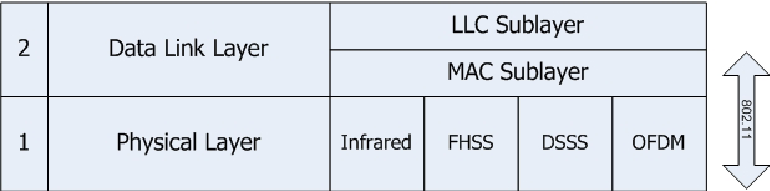
\includegraphics[width=0.9\columnwidth]{graphics/80211_protocol_stack}
	\end{center}
	\vspace{-1em}
	\caption{Layer one and two of the ISO/OSI protocol stack}
	\label{80211standard}
\end{figure}

\begin{description}
    \item[Data Link Layer:] The MAC sublayer is responsible for the access to the wireless medium. Possible access methods are CSMA/CA (Carrier Sense Multiple Access using Collision Avoidance), CSMA with RTS/CTS (Request To Send/Clear To Send) or PCF (Point Coordination Function).
	\item[Physical Layer:] This layer is responsible for transferring bits from one wireless device to another. IEEE 802.11 defines infrared and radio frequency communication. The way how the frequencies are used are either defined in the FHSS (Frequency Hopping Spread Spectrum), the DSSS (Direct Sequence Spread Spectrum) or the OFDM (Orthogonal Frequency Division Multiplexing). For a more detailed explanation see also \cite[p.85-87]{mobile_computing}.
\end{description}


\section{Types and Architectures}

As with the possibility to create networks without using any cables and the fast development of wireless networks there exists the need to create networks that serve specific purposes like setting up a wireless network quickly or serving a lot of users. In general, there exist two major types of networks, {\em independent \ac{BSS}} and {\em infrastructure BSS}, whereas the latter has several subtypes which are described briefly.

\subsubsection{Independent BSS (IBSS)}

Often these networks are also called {\em ad hoc networks} because they can be set up very quickly using simple WLAN cards without the need of any additional hardware. This type of network is set up for specific purposes like meetings, conferences or LAN parties and exists only over a short period of time. All participants communicate directly with each other. As figure \ref{ibss} shows there is no intermediate station that is responsible for managing the connections of all stations like it is the case in infrastructure networks.

\begin{figure}[htbp]
	\begin{center}
		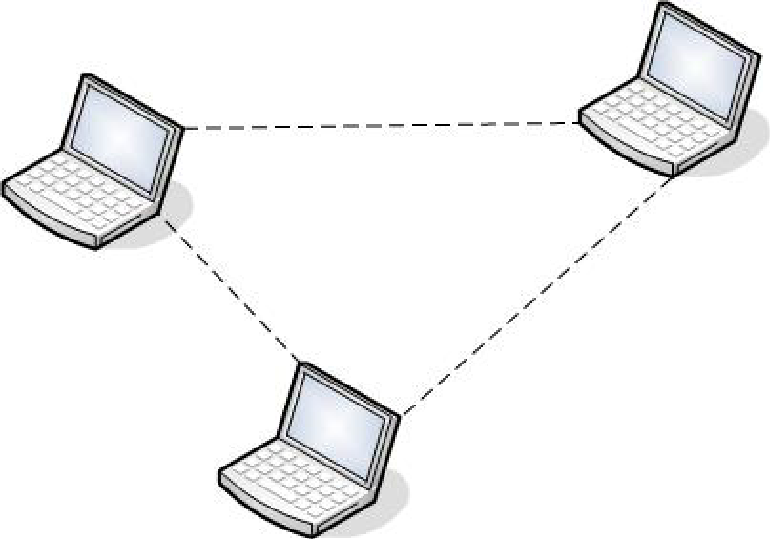
\includegraphics[width=0.5\columnwidth]{graphics/IBSS}
	\end{center}
	\vspace{-1em}
	\caption{An IBSS. All clients are connected directly}
	\label{ibss}
\end{figure}

\subsubsection{Infrastructure BSS}

The difference between an IBSS and an infrastructure BSS is that the latter uses an access point which serves as a central station that handles associations and data for all participants and is "a bridge to the wired network" \cite[p.5]{wildpacket}. Figure \ref{infrastructurebss} shows a sample infrastructure BSS configuration. Whenever a participant of the network wants to send data to another host it first sends the data to the access point which then forwards the data to the desired destination. An infrastructure BSS has some advantages over a simple ad hoc network:

\begin{itemize}
    \item Due to the fact that every station sends the data packet to its associated access point which then forwards it to its destination the covered area of the wireless network is specified by 
		the access point and not by the participants
	\item In case a station is in power saving mode the access point can 
		buffer the received packets for the destined client. As soon as the sleeping station comes up again the access point can send the data
	\item In an infrastructure BSS stations first have to associate with the 
		network in order to be able to send and receive data to and from the network. 
		The access point can accept or deny the association attempt of a station 
		based on parameters that can be set in the access point. For example 
		most access points have ACLs which are used to block certain \ac{MAC address}es
\end{itemize}

\begin{figure}[htbp]
	\begin{center}
		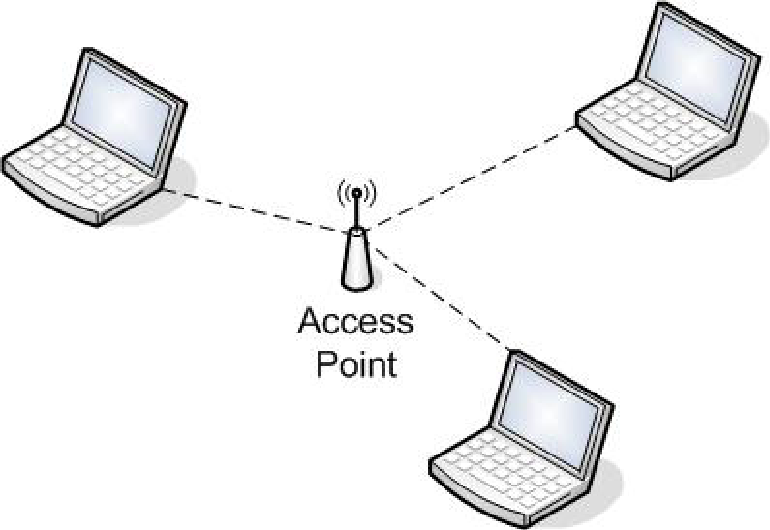
\includegraphics[width=0.5\columnwidth]{graphics/InfrastructureBSS}
	\end{center}
	\vspace{-1em}
	\caption{An infrastructure BSS. The access point manages all stations}
	\label{infrastructurebss}
\end{figure}

\subsubsection{Extended Service Set}

As the covered area in a simple infrastructure BSS is limited by the power of one single access point an extended service area can cover larger areas by using a lot of access points that are linked together. By giving every single access point the same \ac{SSID} huge wireless networks can be created. A distributed system is responsible for delivering the data from one access point to another. This network topology offers the possibility for stations to move around and change the associated access point while staying connected. The wireless card takes care of connecting to the access point with the highest signal strength.\footnote{The access point with the highest signal strength is normally the nearest one}

\subsubsection{Multi-BSS or "Virtual Access Points"}

Some access points offer the possibility to create two or more BSS, each with 	different privileges. For example in a company there would exist a network with the name "company" that would be used by the people working in the company. Additionally, there would exist another network with the name "guest" which could be used by the people that do not work in the company. Both networks would be managed by the same access point. The network with the name "company" could be secured using \ac{WEP} or \ac{WPA} and could grant access to privileged users only. The network "guest" would offer access to every person who has a WLAN card but the access to the network should be more restricted. As a consequence the access point would handle the requests coming from a certain station differently. It would either forward to the internal company network or would give only access to the guest network \cite[p.19]{80211wireless}.
\pagebreak
\section{Specification of WLAN Frames}

Each single frame sent in a wireless network has a certain structure. The general format of an IEEE 802.11 frame and a description including the size of each field in bytes is shown in figure \ref{frameformat}. A frame is transferred from the left to the right with respect to time.

\begin{figure}[htbp]
	\vspace{1.5em}
	\begin{center}
		\includegraphics[width=\columnwidth]{graphics/GeneralMACFormat}
	\end{center}
	\vspace{-1em}
	\caption{Format of an IEEE 802.11 WLAN packet. Sizes in byte}
	\label{frameformat}
\end{figure}

\subsubsection{Frame Control}

The Frame Control part of each packet is split up into several subfields as shown below in figure \ref{framecontrol}.

\begin{figure}[htbp]
	\vspace{1.5em}
	\begin{center}
		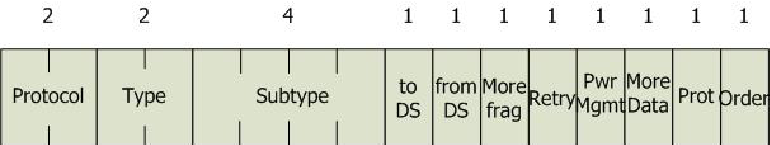
\includegraphics[width=0.75\columnwidth]{graphics/FrameControl}
	\end{center}
	\vspace{-1em}
	\caption{Frame Control of an IEEE 802.11 WLAN packet. Sizes in bit}
	\vspace{1.5em}
	\label{framecontrol}
\end{figure}

The value of the {\bf{\em Protocol}} field indicates the version of the 802.11 MAC. Until now, there exists one version with the value 00b.

The {\bf{\em Type}} and {\bf{\em Subtype}} fields of the Frame Control indicate what kind of information is sent over the network. There exist three types of frames named {\em Management frames} (responsible for authentication, association and disassociation of clients, synchronisation, etc.), {\em Control frames} (responsible for RTS/CTS procedure, acknowledgements of received frames, power saving of access points, etc.), and {\em Data frames} (responsible for data, QoS, etc.). These two fields play a major role when implementing a wireless tool because based on this information the program has to interpret the data following the Frame Control field. See \cite[p.36]{80211standard} for a list with all possible values and their meaning. \\

The {\bf{\em to DS}} and {\bf{\em from DS}} fields indicate whether data is coming from or going to a distributed system. Table \ref{tofromDS} shows detailed information about the different ways these values can be set and their meaning. See also \cite[p.49]{80211wireless}.

\begin{table}[htbp]
	\begin{center}
		\vspace{1.5em}
		\begin{tabular}{l|p{100pt}|p{100pt}}
		&\bf{to DS = 0b}&\bf{to DS = 1b}\\
		\hline
		\bf{from DS = 0b}&All frames in an IBSS&Data frames sent from a station
			to the DS\\
		\hline
		\bf{from DS = 1b}&Data frames coming from the DS&Frames on a WDS
			(wireless bridge)\\
		\end{tabular}
	\end{center}
	\caption{Possible settings for the {\em to DS} and {\em from DS} fields}
	\vspace{1.5em}
	\label{tofromDS}
\end{table}

In case the {\bf{\em More fragments}} bit is set to 1b the current frame is fragmented. Each fragmented frame, excluding the last one, set it to 1b. The most common case is that no fragmentation is used, so this field would be set to 0b.

In case frames have to be transmitted more than once (for instance when a frame gets lost) the value of the {\bf{\em Retry}} field is set to 1b. Otherwise it has the value of 0b.

The {\bf{\em Power management}} field tells whether a mobile station is in power saving mode.

The {\bf{\em More Data}} field indicates whether the access point buffers data for a sleeping station which is in power saving mode.

In case a frame is protected by an upper layer protocol (for instance WEP) the {\bf{\em Protected}} bit is set to 1b. This is necessary because in case the frame is encrypted its structure might change a little bit.

In case frames have to be transmitted as a sequence, the {\bf{\em Order}} field is set to 1b. It is important to note that setting this bit to 1b means more computation overhead for each WLAN card involved.

\subsubsection{Duration/ID}

This field can have different meanings. First, it can be an indication for how long the wireless medium will be reserved for a transaction of frames. Next, it can be used for telling all stations that a contention free period has started. Finally, it can also be used by the stations to tell the access point to send buffered frames when a station leaves its power saving mode.

\subsubsection{Address fields (Address 1 to 4)}

Depending on the values set in the {\bf{\em to DS}} and {\bf{\em from DS}} field in the Frame Control part three or four address fields can be set. The meaning of the different address fields is as follows: Address 1 is the receiver of a frame, Address 2 the transmitter of a frame, Address 3 is used for filtering depending on the receiver and type of the network and Address 4 is used only in wireless bridges and is not discussed here. Each address is a 48 bit MAC address identifier.

In case all bits of an address are set to 1b (FF:FF:FF:FF:FF:FF) then it is a broadcast address which means that the frame is sent to every station in the network.

In case it starts with a 0b (for instance 00:03:4A:72:FC:31) then it is a unicast address which points to one single station.

There exist other types of addresses which can be viewed at \cite{mac_meaning}.

\subsubsection{Sequence Control}

"This 16-bit field is used for both defragmentation and discarding duplicate frames. It is composed of a 4-bit fragment number field and a 12-bit sequence number field" \cite[p.52]{80211wireless}. Each frame has an own sequence number. In case a frame is fragmented the fragment number is incremented by one but the sequence field stays the same.

\subsubsection{Frame Body}

This field contains the payload of a frame.

\subsubsection{Frame Check Sequence}

A station can check the received frame for its correctness. The check is done by using a \ac{CRC}. All fields of the frame are included in the check. The CRC is done before a frame is sent from the sending station and before it is processed by the receiving station. %The receiver compares the value in the FCS field with the result of its own CRC.

\section{Hidden Node Problem}
\label{sec:hidden_node_problem}

In a wireless network it is possible that not every station is in range of all others. As it is shown in figure \ref{hiddennode} it is possible that one client (the access point in this example) can be in range of station 1 and station 2 but station 1 may not be in sending range of station 2. This means that it is not possible for station 1 to determine whether station 2 is currently sending or not and vice versa. This is called the {\em hidden node problem}.

\begin{figure}[htbp]
	\vspace{1.5em}
	\begin{center}
		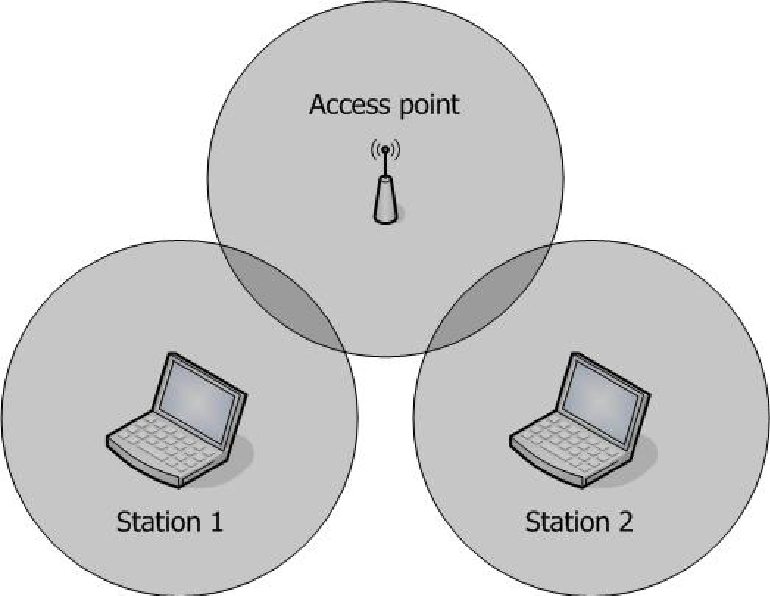
\includegraphics[width=0.5\columnwidth]{graphics/HiddenNode}
	\end{center}
	\caption{The hidden node problem}
	\vspace{1.5em}
	\label{hiddennode}
\end{figure}

To overcome this problem when using a wireless medium CSMA with RTS/CTS is used to make sure that the medium is idle. By using a four way handshake in which particular frames are exchanged all participants of a wireless network get informed whether the medium is idle and possible for a transfer or not. This handshake is done by sending RTS (Request To Send) and CTS (Clear To Send) frames. Figure \ref{rtscts} was taken from \cite[p.36]{80211wireless} and illustrates the process of how a sender and receiver communicate RTS and CTS frames before sending data and its acknowledgement.

\begin{figure}
	\begin{center}
		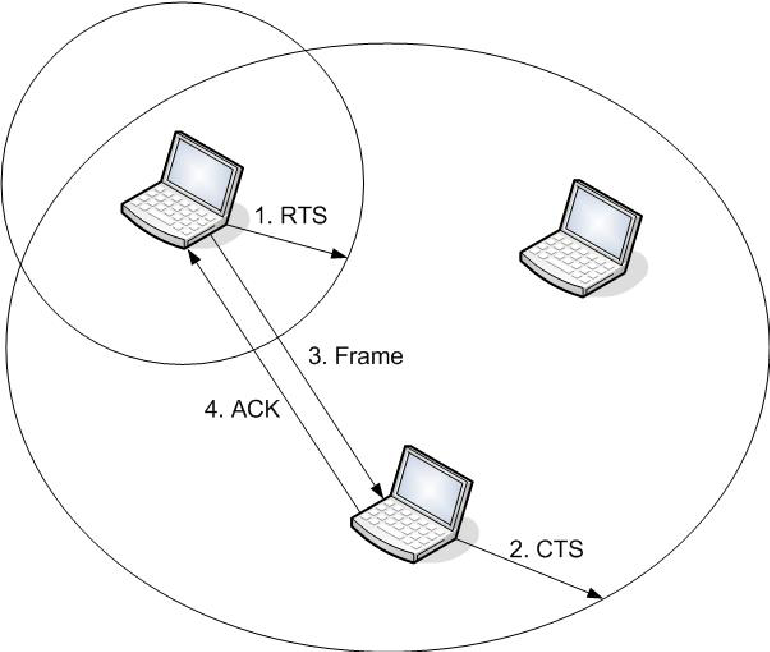
\includegraphics[width=0.65\columnwidth]{graphics/RtsCtsHandshake}
	\end{center}
	\vspace{-1em}
	\caption{The RTS/CTS handshake}
	\vspace{1.5em}
	\label{rtscts}
\end{figure}

Since the fact that this four way handshake requires a lot of additional frames sent over the wireless medium it is only used in large company environments where the probability of interfering sending stations is more severe. In smaller environments the handshake procedure is not performed and the data is simply sent without worrying about the hidden node problem. If simultaneous transmissions happen then the frame, on which the collision happened, is simply resent.

\section{Producing Traffic}

Before a station can send and receive data in a wireless network a client has to go through the authentication and the association process. According to \cite{authassoc} the process of connecting to a wireless network is split up into three phases.

\subsubsection{Phase 1: Probing}

A station in this phase is neither authenticated nor associated. It checks its environment for possible access points which it can connect to.

\subsubsection{Phase 2: Authentication}

After the station found an access point it authenticates itself to the network. There exist two ways on how to do this. If the access point uses {\em open} authentication, a new station can associate with an access point without taking any additional steps. The other possibility is {\em shared} authentication. Using this technique some encryption mechanism like WEP is used. A client has to provide a secret key to authenticate to a network successfully.

\subsubsection{Phase 3: Association}

After a station was authenticated successfully it has to associate with the access point. The association of a new station is always initiated by the station. In order to associate with an access point it is necessary to determine the SSID, which is the name of a wireless network. To simplify the location of wireless networks an access point can periodically send out beacon frames which are received by all stations in range. The information kept in beacon frames also includes the SSID. A station collects a beacon frame, extracts the SSID and sends an association request to the access point. If the wireless network is in {\em hidden mode}, it does not send any beacon frames which could be collected by clients. In this mode a new client of the network has to know the SSID in advance.

After a successful association a station can send and receive data to and from the wireless network.


\chapter{Network Scanning}

\section{Introduction}

In order to be able to infiltrate a wireless network it is necessary to gather information about the network and its properties. This can either be done by being a legitimate client and knowing a lot of things about the network beforehand or by using wireless network scanners which scan the network and display the information needed. As described later wireless tools present information about a network to the user. Useful information which can be gathered by a simple wireless scanner include:

\begin{description}
    \item[SSID:]
		In case of a cloaked network it is not possible without the
		knowledge of the SSID to associate with a network. SSIDs can be received
		in two ways. One way is to collect beacon frames which are automatically sent out by an access point. So the only thing a cracker has to do is to wait for an incoming beacon frame and read out its SSID information. If the access point does not send out beacon frames, a cracker has to
		wait for a probe request of a new legitimate station which includes the SSID information of the network it wants to connect to.
	\item[DHCP information:]
		In case a wireless network is found, either by receiving a beacon frame
		or a probe response in a cloaked network, the next step is to find
		out whether there exists a DHCP server in the network. If there exists
		one or more DHCP server in the network, a cracker simply broadcasts a
		DHCP discover request to the network and receives all information that is
		required. Although it is easier for the network administrator to
		set up a DHCP server than assigning static \ac{IP} addresses it is critical
		to use DHCP because the person who infiltrates the network
		probably knows about the simplicity of using the DHCP service.
	\item[IP information:]
		For a successful login it is necessary to know on which IP addresses a 
		network operates and the address of the gateway. This can be done by 
		capturing data frames that contain IP information like ARP, TCP or UDP 
		frames.
	\item[MAC addresses:]
		Each single network card has its worldwide unique MAC address. By 
		configuring the access point to accept only association attempts from devices with MAC 
		addresses that are known it is impossible for an 
		intruder to enter a wireless network in case the MAC address of the 
		\ac{NIC} owned by the intruder is not spoofed. MAC addresses can be read 
		out of every single packet that is sent over the network.
	\item[Encryption:]
		Most access points still use WEP encryption. After the 
		RC4 algorithm was cracked by Scott Fluhrer, Itsik 
		Mantin and Adi Shamir (see \cite{rc4weak}) a new encryption method was developed (WPA) and should be used 
		in a wireless network environment because it is still considered secure. %In case a network is not encrypted at all it is a matter of minutes for a cracker to break in. Otherwise it takes at least a couple of hours when using the simplest WEP encryption.
	\item[Uptime:]
		By knowing the period of time an access point is online a cracker can find out 
		whether the access point is disabled in the nights or whether it 
		runs over weeks without being set offline which indicates a lack of 
		security. In general it is not common that a network operator 
		monitors the networks during the nights. The uptime information is located in a beacon frame.
	\item[Signal strength:]
		\cite{signal_strength} describes it as "a signal ... that indicates the strength of the incoming (received) signal in a receiver". The higher the signal strength the faster the connection. 
		When sitting close to an access point the probability to receive 
		certain frames is much higher than sitting at the edge of its covered area. This 
		information is located in the private headers of a packet and can only be read out of certain chipsets like Prism WLAN cards.
\end{description}

\section{Active versus Passive Scanning}
\label{sec:active_passive_scanning}

The first way of scanning a wireless network is named {\bf {\em active scanning}}. By using packet injection an active wireless network scanning software sends probe requests leaving the SSID field empty to the wireless medium. In case an access point is not in hidden mode it responds with a probe response including the SSID. The problem of this approach is that networks which are in hidden mode can not be found and so stay unknown for the user. Another drawback of this method is that packets have to be sent and as a consequence information about the software and the scanning client is revealed. Information that can be gathered includes the MAC address which can identify a wireless network card uniquely, its signal strength or even the software used. The latter piece of information can be retrieved by using fingerprinting techniques. According to \cite{triangulation} it is even possible to physically locate active scanners by using triangulation.

When using {\bf {\em passive scanning}} the wireless NIC is first set into {\em monitor mode}\footnote{It is also called {\em promiscuous mode} or {\em rfmon}. That means a card can be put in a mode in which it can capture all packets that travel through the air. Even those packets are captured that are not destined for the scanning NIC.} and then scans the air. That means that these tools can also find hidden networks because they can capture traffic from another station to an access point. On the other hand it is not possible with standard hardware to send out any packets. As a consequence it is only possible to scan a network but not to inject packets. Tools using the passive scanning technique can neither be located nor identified.

\section{Wardriving}

"Wardriving, also called access point mapping, is the act of locating and possibly exploiting connections to wireless local area networks while driving around a city or elsewhere." \cite{wardrivingdef}

In order not to confuse wardriving with the original meaning of the word {\em war} today it stands for {\bf W}ireless {\bf A}ccess {\bf R}evolution. The second part of the term indicates the type of transportation. 

Beside wardriving there exist a lot of modifications like {\em warwalking} (walking around with a laptop), {\em wartraming} (scanning networks inside a tramway), {\em warbiking} (scanning networks while riding a bike), etc. Due to the different possibilities to move around the act of searching for wireless networks is sometimes named {\em warXing}.

The topic wardriving came up around the year 2000. Peter Shipley claims being the inventor of wardriving. See \cite{shipley} for a brief portrait. He and others were the first persons who pointed the finger on the insecurities of wireless networks and started to create scripts that automated scanning for wireless networks. The initial idea was to map positions of wireless networks on maps to show how many of them are open or secured by WEP.

From these days on a lot of different tools were developed which became more and more powerful and people started to misuse wireless networks they found for their own purpose.

\section{Warchalking}

"The act of making chalk marks on outdoor surfaces (walls, sidewalks, buildings, sign posts, trees) to indicate the existence of an open wireless network connection, usually offering an Internet connection so that others can benefit from the free wireless access." \cite{warchalkingdef} Figure \ref{warchalk} shows a table with possible warchalking signs.

\begin{figure}[htbp]
	\vspace{1em}
	\begin{center}
		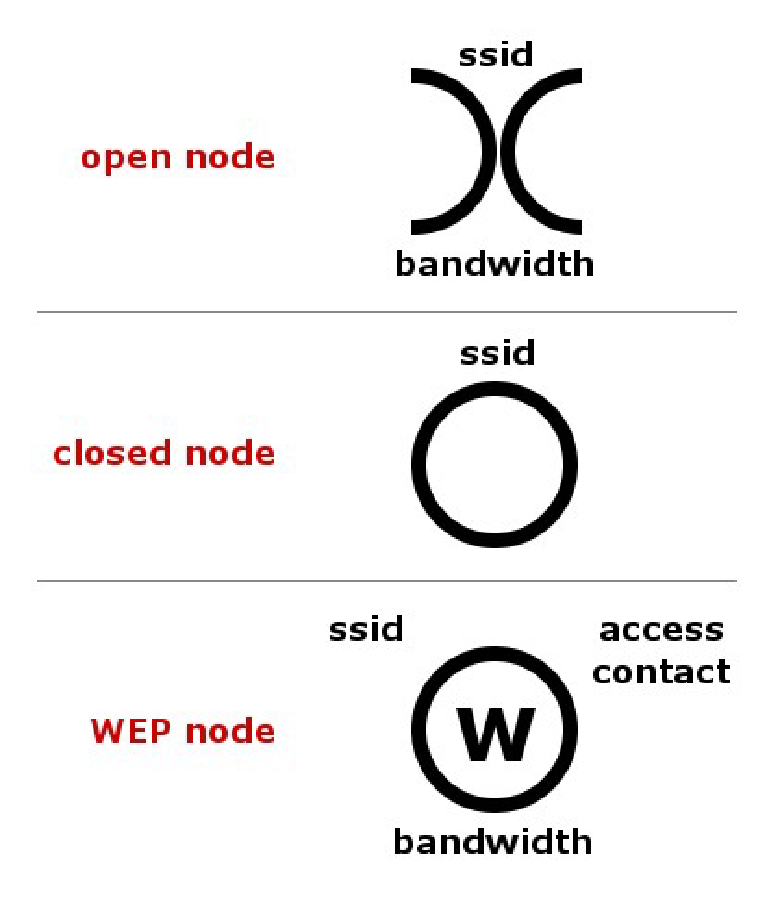
\includegraphics[width=0.45\columnwidth]{graphics/Warchalk}
	\end{center}
	\vspace{-1em}
	\caption{Warchalking signs \cite{warchalkingimg}}
	\label{warchalk}
\end{figure}

The symbols on the right side indicate the sign which is painted on a wall to inform about a particular type of network. The information put in each symbol tells enough about the effort that is necessary to gain access to a network. Later in this work it is shown that an open network is much easier to infiltrate than a network that is WEP protected.

\section{Equipment}

The standard equipment of a wardriver typically consists of a laptop and a wireless network card. Often a GPS antenna is also used to generate maps showing all access points found including additional information like the signal strength or encryption information. Due to the fact that the coverage of a wireless NIC is limited some wireless cards have the capability to add external antennas to improve their receiving range. As a result more wireless networks can be found.

Depending on the way networks are scanned there exist different types of operating systems and chipsets of wireless NICs which have different capabilities.

For a normal scan of a wireless network it is sufficient to use any wireless NIC and Windows as the operating system. There is no need for special software because Windows has a built in wireless network scanner. Besides, there exist powerful scanning software for this \ac{OS}.

A lot of wireless network scanners are available for Linux and monitor mode is supported for a large range of chipsets.\footnote{See \url{http://www.linux-wlan.org/docs/wlan_adapters.html.gz} for a complete list with all vendors and chipsets of different wireless NICs.} Common chipsets include Prism, Orinoco and Aironet because the usage of their monitor mode is easy and a lot of tools written in Linux can set and unset the monitor mode automatically.

\section{Ethics}

According to \cite{wardrivingforms} the actual goal of a wardriver can generally be classified in three different groups:
\vspace{-0.5em}
\begin{enumerate}
    \item The first group simply wants to create maps for cartographic and statistical purposes
	\item The second group makes fun out of finding wireless networks and practices warchalking to inform other wardrivers of available networks
	\item The third group is the most dangerous one. These people search, find and misuse wireless networks for their own purpose. In Austria this group is acting against the law and can be punished for its actions (see the following section \ref{sec:laws} for details)
\end{enumerate}

\section{Laws}
\label{sec:laws}

As companies and individuals begin to realise that wardriving costs companies millions of Euros every year\footnote{An article available at http://www.securitymanagement.com/library/001493.html speaks of approximately 70 million dollars a year} it becomes necessary to create laws that prevent wardriving. The biggest problem to create such laws is that computer industry is a very fast evolving area of science compared to law and legislation which is a slow process. New laws have to be discussed and validated which takes a lot of time. Nevertheless in august 2003 a new communication law passed in Austria.

The law says that it is prohibited to listen in, eavesdrop, record or intercept communicated messages as well as the transfer of scanned data to third persons. In case someone receives messages that are not intended to be received by this person then this data has to be deleted immediately.\footnote{BG BGBl. I 2003/70 � 93 section 3, 4}

On the other hand the operators of wireless networks are addressed. It is to the same amount illegal to operate a network that is insecure. The law says that an operator has to take care of the data protection of all users using a wireless network. That means an operator has to make arrangements for anyone using the network so that an abuse is not possible. The operator of an insecure network can be charged with up to 4000 Euro.\footnote{BG BGBl. I 2003/70 � 78 section 2}


\chapter{Wireless Intrusion Detection}

\section{Definition}
\label{sec:wids_definition}

An {\em intrusion detection system} (\ac{IDS}) is a piece of software that knows how to detect intrusion attempts and unusual behaviour in a network. It possibly performs counter actions on a specific user who infiltrates the network. For a more detailed definition see also \cite{idsdef}.

The underlying study discusses only {\em network based systems} and ignores {\em host based systems} since they are not relevant for this work.

\section{Passive versus Reactive Systems}

A way to classify different IDS is to distinguish the reaction that is taken when an intrusion attempt of a user is detected. In a passive system no active reaction is taken. The administrator just gets informed about a malicious user and logs are created. In a reactive system the IDS responds to an intrusion attempt by issuing active counter measures. For instance it could log off the user or update the firewall to lock the malicious user out of the network.

\section{Signature versus Anomaly Based Systems}
\label{sec:sig_anom_ids}

As shown in \cite{idsdef} IDSs can also be classified by focusing on the techniques used to detect abnormal behaviour. There exist two different approaches on detecting a misuse:

\begin{description}
    \item[Signature based:] A signature based system contains a database with signatures of known attacks on a network. Whenever frames are received the system compares the signatures stored in the database with the signature created for the received frames. If the signatures are equivalent, an attack is detected and an alert is created. A signature is either a single action (i.e.: a login to a system) or a sequence of actions.

"The advantage of this method is that there are few false alarms, or false positives, when attacks are detected" \cite[p.9]{wids}.

On the other hand the whole system is only as good as the underlying database. If the status of the signature database is outdated, the system is not able to detect new attacks since these signatures are not available. Besides, variations of known attacks can not be discovered since their signature differs from the original one.

	\item[Anomaly based:] In an anomaly based system a network administrator defines parameters that define the {\em normal behaviour} of the network. For example in order to detect flood attacks thresholds which identify the maximum number of packets in a particular period of time can be set. Another example are white lists of known clients which are allowed to use a network. In case a client with an unknown MAC address appears it is probably a malicious user. The advantage is that unknown attacks can be detected. On the other hand the quality of the system relies on the values defined by the administrator. Very often more false alarms are created when using an anomaly based system than when using a signature based system \cite[p. 3]{IDS_anomaly_false_alarms}.

\end{description} 

\section{Structure of an IDS}
\label{sec:ids_structure}

Different IDS provide the user with a varying amount of features. Despite the big differences in capabilities of each IDS the basic structure stays the same. It is generally divided into four parts described below. See \cite{wids_schreiber} for more information.

\begin{enumerate}
    \item The {\bf {\em data gathering component}} is responsible for collecting data that is transferred over the network. This component is called {\em sensor} or {\em drone}. It transmits the received data to the data processing component
	\item The {\bf {\em data processing component}} is the core of an IDS. It compares all received data and tries to detect attacks
	\item The {\bf {\em data storage component}} stores the data that was already processed and makes it available at a later time
	\item If an attack is discovered, the {\bf {\em response component}} performs counter measures like logging off a user
\end{enumerate}

\section{Security Aspects}

According to \cite{wids_schreiber} an IDS is an interesting goal for a cracker. As a consequence the IDS itself has to be protected from the following threats:

\begin{description}
    \item[\ac{DoS} attack:] Since the IDS scans and stores packets that are relevant for the detection of an attack a cracker could send out large amounts of these packets to bring the IDS down. A counter measure to this threat is to use a buffer which overflows when it is full. The data processing component takes the data from this buffer instead from the data gathering component directly. The drawback of the buffer is that at the time the buffer is full the system can not respond to attacks that are currently running
    \item[Direct attack:] Since programs (especially those written in C/C++ 
where pointers are used) are vulnerable to buffer overflow attacks the IDS can be brought down by such an attack. The difference to the DoS attack described above is that the direct attack tries to exploit the weaknesses in the code of the program. The DoS attack tries to harm the system based on its function, namely intrusion detection
	\item[Communication channel attack:] This attack deals with disturbing the communication between the IDS and its infrastructure. An example is a cracker who manages it to bring down the mail server which sends out alerts and warnings to the network administrator
	\item[Subterfuge attack:] "In a subterfuge attack, an attacker attempts to mislead the monitor as to the meaning of the traffic it analyzes" \cite{subterfuge_attack}. For instance in an anomaly based system the cracker performs the attack very slowly so that the IDS does not recognise it

\end{description}


\chapter{Neural Networks}

\section{Introduction}

This section gives an overview of neural networks. First, the difference between biological and artificial neural networks (\ac{ANN}) is explained. Next, artificial neural networks are explained in more detail by showing different learning methods. Additionally, some learning algorithms are shown like the principles of {\em delta rule learning} and {\em backpropagation learning}.

\section{Definition}

\cite[p. 156]{essence} states that a "neural network consists of many simple processing units (or neurons) connected together. The behaviour of each neuron is very simple but together a collection of neurons can have sophisticated behaviour".

\section{Biological Neural Networks}

The basis of an artificial neural network is the human brain. A brain consists of billions of simple processing units called neurons. Each neuron is connected with thousands of other neurons over axons and dendrites. Figure \ref{singleneuron} shows one single neuron. The communication in a neural network takes place over the connections named axons (output of the neuron) and dendrites (input to the neuron). Whenever the received input stimulation exceeds a certain threshold the neuron becomes activated, fires and gives its output to its neighbouring neurons. The receiving neuron again checks for the threshold and so on.

\begin{figure}
	\begin{center}
		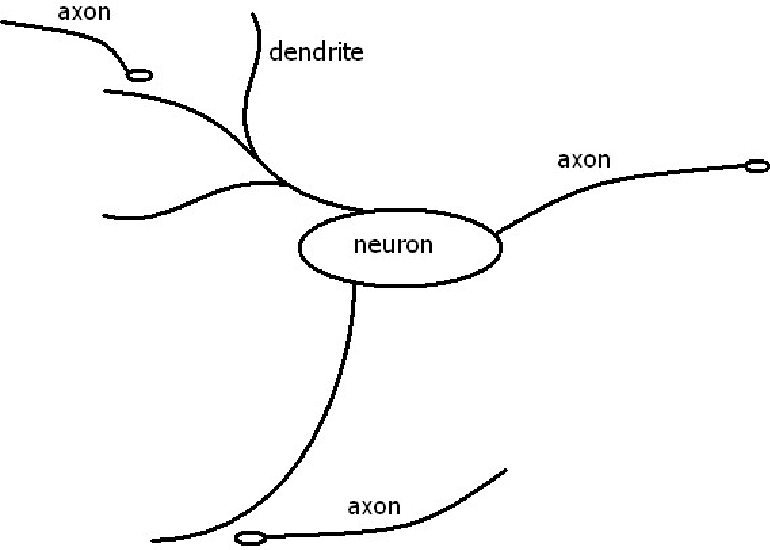
\includegraphics[width=0.75\columnwidth]{graphics/HumanNeuron}
	\end{center}
	\vspace{-1em}
	\caption{One neuron of the human brain}
	\vspace{1em}
	\label{singleneuron}
\end{figure}

The learning process of the human brain depends on the synapses. When a synapse receives input it releases certain chemicals in order to forward to the next input. Depending on the amount of chemicals released the received stimulation is forwarded by a certain strength. Learning is done by adjusting this amount \cite[p.157]{essence}. As described in the next section in an artificial network this amount of chemicals can be illustrated by using weights between neurons.

\section{Artificial Neural Networks}

The idea of creating neural networks with weighted connections came up around 1960 when Frank Rosenblatt published his paper {\em Perceptron}. He was one of the pioneers who developed and coined the term {\em perceptron} which became the basis for today's neural networks. For detailed information about Frank Rosenblatt see also \cite{rosenblatt} and \cite[p.55]{neuralnetworks}.

\subsubsection{Capabilities of ANNs}

An ANN can be used for complex classification tasks and will most likely find good solutions for a large range of problems. Besides, after it is trained to solve a specific problem it can find solutions for other similar problems. The following list shows some areas where ANNs can be used. See also \cite{nn_applications}.

\begin{itemize}
    \item Pattern recognition (characters, images, etc.)
	\item Language processing
	\item Complex logical operations
	\item Data compression
	\item Optimisation
	\item Simulation
\end{itemize}

\subsubsection{Drawbacks of ANNs}

ANNs suffer from some drawbacks. See also \cite{nn_limitations}.

\begin{itemize}
    \item The quality of the results depends on the features chosen to train and use the network and the input values
	\item The weights of a network store the information implicitly. That means it is not possible to understand the values of the weights in a network
	\item The processing time needed to solve a problem grows as the problem size grows
\end{itemize}

\section{Activation Functions}
\label{sec:activation}

The activation function of a neural network describes how the output of a neuron is calculated. The most common ones used are described in the following section \cite{nn_actfct}.

\begin{description}
	\item[Hard limiter:] This function is described mathematically as
\begin{equation}	f(x) =
	\begin{cases}
		1 & \text{if } x \ge 0 \\
		0 & \text{otherwise}
	\end{cases}
\end{equation}
It says that every time the argument $x$ of the function $f(x)$ is greater or equal to zero the output of the neuron is $1$. Otherwise it is $0$. See also \cite[p.178]{pattern}.

	\item[Identity:] This function is described as
\begin{equation} y = Cx \end{equation}
where $C$ is a constant and is mostly 1. The derivative is simply $C$.

	\item[Sigmoid:] This function is described as \begin{equation} y = \frac{1}{1+\exp(-ax)} \end{equation}
where $a$ is a value that changes the shape of the sigmoid function. The higher this value, the more it looks like the hard limiter function. The output of this function lies always between $0$ and $1$. The derivative is $y * (1 - y)$. See also \cite[p.149f]{neuralnetworks} and \cite[p.184]{pattern}.

\end{description}

Figure \ref{activation} shows all activation functions in one graph. The sigmoid function uses the value $10$ for the variable $a$.

\begin{figure}[htbp]
	\begin{center}
		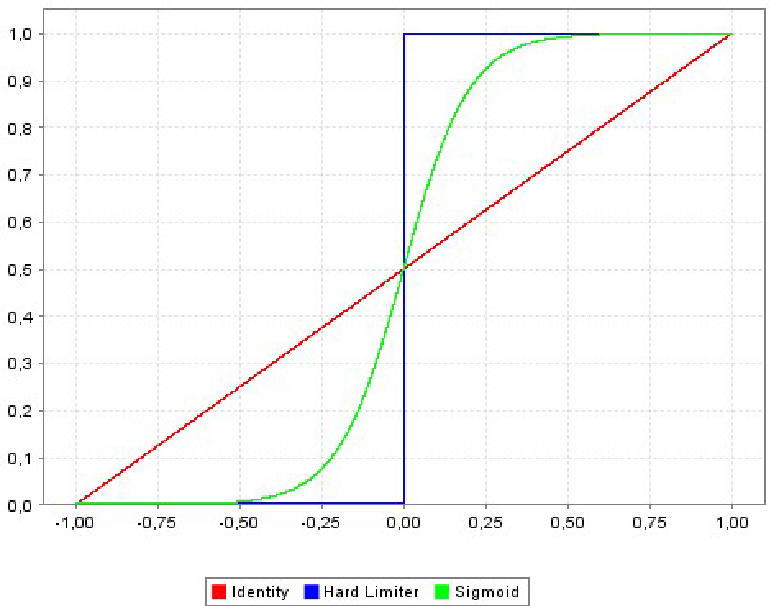
\includegraphics[width=0.55\columnwidth]{graphics/Activation}
	\end{center}
	\vspace{-1em}
	\caption{A graph that shows all activation functions presented}
	\label{activation}
\end{figure}

\section{Perceptron}
\label{sec:perceptron}

As described in \cite[p.178]{pattern} figure \ref{perceptron} shows an idealised perceptron. It consists of input values $x_1,...,x_n$, their respective weights $w_1,...,w_n$ and an output $c$.

\begin{figure}[htbp]
	\begin{center}
		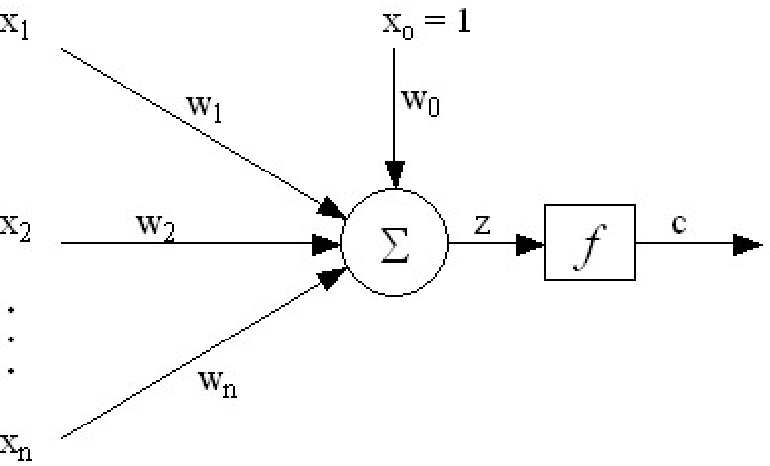
\includegraphics[width=0.55\columnwidth]{graphics/Perceptron}
	\end{center}
	\vspace{-1em}
	\caption{An idealised perceptron}
	\label{perceptron}
\end{figure}

Whenever the perceptron receives input values on its input nodes the values are multiplied with the respective weight and all results are summed afterwards. This process can be shown as \begin{equation} c = f(z) \end{equation} where \begin{equation} z = \sum_{i=1}^n w_ix_i \end{equation} After $z$ is calculated it is given to $f(z)$ which is the activation function of the perceptron. The output of this function is the output of the perceptron. In case the desired output can either be true or false (1 or 0 respectively)  this is a hard limiter function as described in section \ref{sec:activation}.

\section{Learning Methods}

Learning in an ANN can be done in two different ways. The method used depends on the problem that needs to be solved.

\begin{description}
    \item[Supervised:]
		When using {\em supervised learning} techniques the desired output is
		available. Table \ref{logicaland} shows an example of possible input values that are given to the ANN ($x_0$ and $x_1$) and the desired output $o$.
		
		\begin{table}[htbp]
			\begin{center}
				\begin{tabular}{|l|l|l|}
				\hline
				$\bf{x_0}$&$\bf{x_1}$&$\bf{o}$\\
				\hline
				0&0&0\\
				\hline
				0&1&0\\
				\hline
				1&0&0\\
				\hline
				1&1&1\\
				\hline
				\end{tabular}
			\end{center}
			\vspace{-1em}
			\caption{The logical AND operation}
			\label{logicaland}
		\end{table}

		In order to learn the logical AND operation it suffices to use a simple perceptron as shown in section \ref{sec:perceptron}.
		At the time values are attached to the input nodes they are propagated
		through the net and the result is compared with the desired output.
		As we will see later depending on the learning
		algorithm the weights in the network are adjusted using different
		methods.

	\item[Unsupervised:]
		The other possibility to learn is {\em unsupervised learning}. When 
		using this technique the desired output is not available and the resulting output of the trained network can not be predicted. This type of networks is not discussed in this work.

\end{description}


\section{Bias}
\label{sec:bias}

As we will see in the next section learning in a neural network depends on adjusting the weights. Since it is possible that all input values from $x_1,...,x_n$ are zero and as a consequence no learning would take place $x_0$ is introduced (see figure \ref{perceptron}). $x_0$ is a pseudo input which is also called a bias. It is responsible for keeping the result of the summation above zero so that learning takes place even though all other input values are zero.

As a consequence the formula $z = \sum_{i=1}^n w_ix_i$ shown in section \ref{sec:perceptron} has to be modified when learning takes place. The resulting formula looks as follows: \begin{equation} z = \sum_{i=1}^n w_ix_i + w_0 \end{equation}


\section{Learning Algorithms}

The learning success in an ANN depends mainly on adjusting the weights between nodes.\footnote{Other parameters also influence the learning progress. These parameters include the number of nodes in a network or the chosen learning rate which is introduced in the following section} Depending on the method chosen to modify the weights in a network it takes a different amount of time to learn something successfully.

\subsection{Delta Learning}
\label{sec:delta_learning}

The delta learning rule computes the new weight depending on the difference between the desired and the calculated output of the network.

The following formula shows how the weights in the delta rule are updated
\begin{equation} \label{eq:delta_rule} w_p(t+1) =w_p(t) - \rho[\delta_p(i)x(i)] \end{equation}
where
\begin{itemize}
	\addtolength{\itemsep}{-1.5ex}
	\item $w_p(t+1)$ is the new weight between two neurons
	\item $w_p(t)$ is the old weight between the same two neurons
	\item $\rho$ is the learning rate
	\item $\delta_p(i)$ is the error value calculated by the following formula \begin{equation} \delta_p(i) = [c_p(i) - o_p(i)]f'(z_p(i)) \end{equation}
		where $o_p(i)$ is the desired output, $f'$ is the derivative of the activation function, "$z_p(i)$ is the weighted sum of the inputs to the $p^{th}$ output neuron" \cite{pattern} and $c_p(i)$ is the calculated output using the formula already described in section \ref{sec:perceptron} and \ref{sec:bias}: \begin{equation} c_p = f(\sum_{i=1}^n w_ix_i + w_0) \end{equation}
	\item $x(i)$ is the $i^{th}$ value of the input vector
\end{itemize}

The following learning algorithm was taken and adopted from \cite[p.186]{pattern} and shows one learning step in a single layer network when using the delta rule:

\begin{center}

\fbox{\begin{minipage}{255pt}
\begin{enumerate}
	\addtolength{\itemsep}{-1.5ex}
    \item Initialise weight vectors $w_p, p=1,...,k$
	\item Present $x(i)$ to the network
	\item Calculate $c_p(i)$ and $\delta_p(i)$ for each neuron as shown above
	\item Update weight vectors as shown above
\end{enumerate}
\end{minipage}}

\end{center}

Figure \ref{delta_learning_ex} shows an example of delta learning using a learning rate $\rho$ of $0.25$ and the identity as activation function. The weights are initialised randomly with the values 0.3 and 0.6. Table \ref{delta_ex_pattern} displays the input pattern to be learnt.

\begin{table}[htbp]
	\vspace{1.5em}
	\begin{center}
		\begin{tabular}{|l|l|l|}
		\hline
		$\bf{x_0}$&$\bf{x_1}$&$\bf{o}$\\
		\hline
		0&1&1\\
		\hline
		1&0&0\\
		\hline
		\end{tabular}
	\end{center}
	\vspace{-1em}
	\caption{An example pattern to be learnt by the perceptron}
	\vspace{1.5em}
	\label{delta_ex_pattern}
\end{table}

As shown in figure \ref{delta_learning_ex} the only thing that needs to be calculated is $\delta_p(i)$. First, the input is given to the network. As soon as $\delta_p(i)$ is calculated all needed values are inserted in (\ref{eq:delta_rule}). Finally, the next input vector is processed using the updated weight values.

\begin{figure}[htbp]
	\vspace{1.5em}
	\begin{center}
		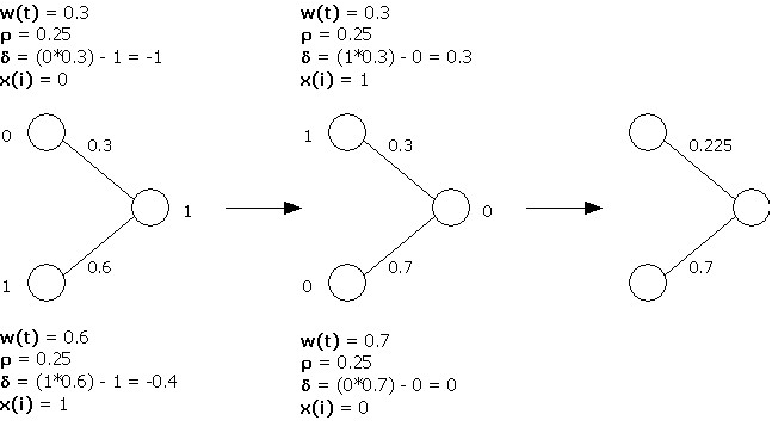
\includegraphics[width=0.8\columnwidth]{graphics/show_delta}
	\end{center}
	\vspace{-1em}
	\caption{An example of using the delta learning rule}
	\label{delta_learning_ex}
\end{figure}

\subsection{Backpropagation Learning}
\label{sec:backpropagation}

A backpropagation network consists of one input layer, at least one hidden layer and one output layer. So that it is possible to update all weights in the network, the weight updating formula shown in section \ref{sec:delta_learning} needs to be extended to
\begin{equation} w^q_p(t+1) =w^q_p(t) - \rho[\delta^q_p(i)c^{q-1}(i)] \end{equation}
assuming that $c^0(i) = x(i)$. Additionally, the computation of the error value has to be divided into two parts. The calculation of the error value for the output layer is
\begin{equation} \delta^L_p(i) = [c_p(i) - o_p(i)]f'(z_p(i)) \end{equation}
and the calculation of the error values for the hidden layer(s) is
\begin{equation} \delta^q_p(i) = [\sum_{s=1}^{k_{q+1}} \delta^{q+1}(i)w^{q+1}]f'(z_p(i)) \end{equation}

The following algorithm shows how learning works when using backpropagation. See also \cite{backpropagation}, \cite{back-propagation} and \cite[p.187]{pattern} for more information.

\begin{center}

\fbox{\begin{minipage}{300pt}
\begin{enumerate}
	\addtolength{\itemsep}{-1.5ex}
	\item Initialise weight vectors $w_p, p=1,...,k_q, q=1,...,L$
	\item Present $x(i)$ to the network
	\item Calculate $c^L_p(i), p=1,...k_L$ as shown in section \ref{sec:delta_learning}
	\item Calculate $\delta^L_p, p=1,...,k_L$ 
	\item For $q = L - 1$ to $1$ do
		\begin{enumerate}
		\vspace{-0.5em}
		\item Calculate the error value $\delta^q_p, p=1,...,k_q$ 
		\end{enumerate}
	\item Update weight vectors
\end{enumerate}

\end{minipage}}
\end{center}

where
\vspace{-1em}
\begin{itemize}
	\addtolength{\itemsep}{-1.5ex}
	\item $L$ is the number of layers in the network
	\item $k_q$ is the number of nodes in the $q^{th}$ layer
	\item $x(i)$ is the input vector
	\item $c^q_p(i)$ is the calculated output value of the $p^{th}$ node in the $q^{th}$ layer
	\item $\delta^q_p$ is the error value of the $p^{th}$ node in the $q^{th}$ layer
\end{itemize}

\input{Analysis}
\chapter{Development of a WIDS}

\section{Overview}

As described in section \ref{sec:wids_definition} the purpose of a wireless intrusion detection system is to detect a malicious client in a network. This chapter shows a concept of a hybrid WIDS which is capable of identifying different threats in a WLAN. Appendix \ref{sec:implementation} shows the tools which are used to create the WIDS and the test environment.

Possible threats include rogue APs, unknown clients, association and disassociation flood attacks. First, the goals of the WIDS are discussed. Then, design details like the classification of the traffic in a network and the process of feature selection is shown. Additionally, an algorithm which finds the best feature set for every problem that needs to be solved is described.

\section{Goals}

The goal of the tool being developed is to create a hybrid WIDS which on the one hand uses well known techniques to detect threats like rogue APs and malicious users. On the other hand it uses a neural network to learn how to identify different wireless threats like association and disassociation floods. The following list shows the main goals of the tool:
\vspace{-0.5em}
\begin{itemize}
	\item It should be possible to use it in every WLAN without worrying about the type of encryption used
	\item Use a neural network to detect association and disassociation flood attacks after a learning phase
	\item The system should be able to react to changes in the characteristics of the network. That means in other words that the WIDS realises when the properties, like the average amount of traffic or the number of connected clients in a network, change
	\item Use white lists to detect rogue APs and malicious clients
	\item It has to be able to receive the input values either from a pcap file\footnote{See glossary} or directly from a capturing NIC. The idea is to perform learning by using a previously stored pcap file. After the learning phase is finished the WIDS starts to capture and analyse packets for intrusion detection

\end{itemize}

\section{Design}

The following sections explain design details of the WIDS, its preprocessor and the process of finding the best feature set for the neural network.

\subsection{WIDS}
\label{sec:design_wids}

The overall design of the WIDS follows the suggested structure presented in section \ref{sec:ids_structure}. Figure \ref{wids_dataflow} shows the four components used and the data flow in the WIDS.

\begin{figure}[htbp]
	\begin{center}
		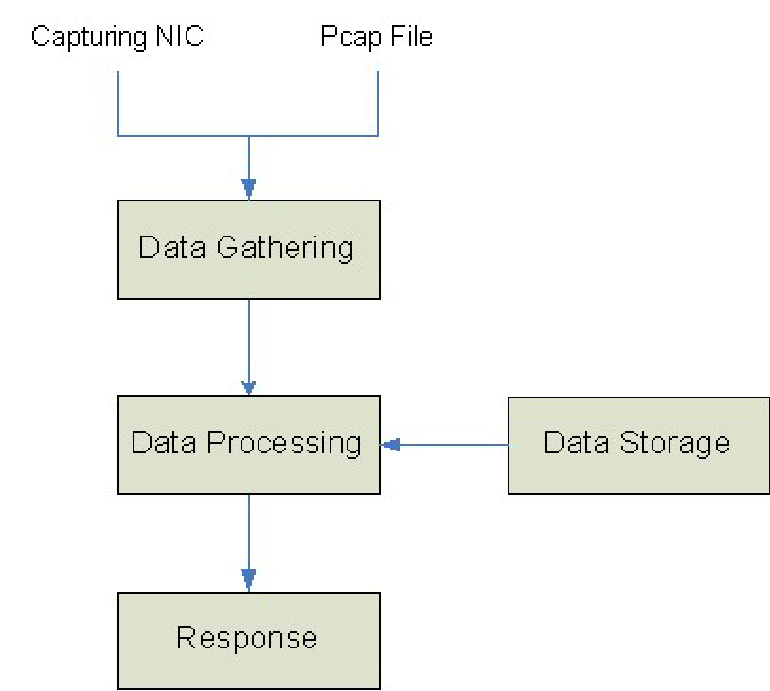
\includegraphics[width=0.7\columnwidth]{graphics/WIDS_structure}
	\end{center}
	\vspace{-1em}
	\caption{Components and data flow in the WIDS}
	\label{wids_dataflow}
\end{figure}

{\em {\bf Data Gathering}}

This component is used to receive data either from a previously stored file or directly from a capturing NIC. The data gathering component forwards the data directly to the data processor.

\pagebreak

{\em {\bf Data Processing}}

The core of the data processing component is a neural network. After training it is capable of identifying association and disassociation flood attacks. It uses the backpropagation learning algorithm described in section \ref{sec:backpropagation}. In addition to the neural network the processor also identifies rogue APs and unknown clients by comparing the content of the white lists created by a preprocessor (described in section \ref{sec:preprocessing}) with the packets received from the data gathering component.

{\em {\bf Data Storage}}

After the training phase this component stores information about a trained neural network. Stored information includes all weights of the network and the {\em scaling values}\footnote{A scaling value specifies the maximum amount of packets with a certain type/subtype that occur in a two second time slot} received. That makes it possible to

\begin{itemize}
    \item create a trained neural network by assigning the stored weight values to the connections between neurons. As a consequence no training phase needs to be done
\vspace{1em}

	\item perform the training phase in several steps. After one training phase is finished it is possible to continue training the network with additional data. This is an important point for the WIDS to be able to react to changes in the network behaviour. The training of the neural network can continue after the initial learning phase is finished by using the data coming directly from the capturing NIC
\end{itemize}

{\em {\bf Response}}

This component is responsible for informing the operator of a WLAN about ongoing threats in the network. The WIDS prints an alert message on the screen.

\subsection{Preprocessing}
\label{sec:preprocessing}

Before the WIDS can be trained several preprocessing steps need to be performed. In order to be able to perform these steps the preprocessor requires a pcap file with normal traffic and one or more files which contain flood specific traffic.

The preprocessor creates white lists for rogue AP and malicious user detection. These lists store the BSSID of every network and the MAC address of every client found inside the normal traffic file.

It addition to the white lists the preprocessor creates additional pcap files (named {\em relevant files}) which are used by the neural network in order to learn the characteristics of different flood attacks. A prototype implementation of the WIDS, which used only the normal traffic file and the flood files to learn, showed, that the neural network does not succeed in learning the characteristics of a flood attack. The reason for that is that association and disassociation packets occur very rarely compared to other packets. As a consequence the neural network would learn too slowly. The relevant files are created out of the normal traffic files and contain only those data packets with the type and subtype field that also occur in the respective flood file.

As soon as these preprocessing steps are finished the network can be trained. The training requires a pcap file with normal traffic, all relevant files and all files which contain flood specific traffic. 

\subsection{Features}

"Since the ability to identify the important inputs and redundant inputs of a classifier results in reduced problem size, faster training and possibly more accurate results, it is critical to be able to identify the important features of network traffic data for intrusion detection in order for the IDS to achieve maximal performance" \cite{nn_features}. That means in other words that the quality of the neural network does not solely depend on the number of hidden layers or neurons used but also on the input features\footnote{A feature is for example the amount of traffic sent to a client or the number of connections coming from the same host in a specified period of time} chosen.

\subsubsection{Feature Selection}
\label{sec:features}

The group of features used as inputs for the neural network is divided into two different sections:

\begin{description}
    \item[Time irrelevant features:] This type of features includes all values that are available by dissecting one single frame. These features do not consider the time aspect. All values are converted to binary values and then given to the neural network.

	\begin{itemize}
	    \item Type field
		\item Subtype field
		\item Retry field
	\end{itemize}

    \item[Time based features:] This type of features takes the period of time that passed since a specific event that happened in the past into account. The WIDS uses two features of this type:

	\begin{itemize}
		\item The number of frames with a certain type and subtype in the past two seconds. This feature is needed to detect association and disassociation floods. The higher this number is the more probable it is that an attack occurs. When given to the neural network this value is scaled from $0$ to $1$ by using the scaling value as divisor. In case the resulting value is bigger than $1$ it is set to $1$. This formula is written as

\begin{equation}
\frac{number\ of\ same\ packets\ in\ the\ past\ two\ seconds}{scaling\ value\ of\ that\ packet\ type}
\end{equation}
\vspace{-0.5em}
		\item The number of disassociations of legitimate clients in the past two seconds. This feature is needed due to the fact that a disassociation flood is harmless in case the source address of the packet is never used in the network. For that reason this feature is needed which checks for packets with a source address of legitimate clients. Again, when given to the neural network this value is also scaled from $0$ to $1$ by using the maximum number of legitimate clients as divisor. This formula is written as

\begin{equation}
\frac{number\ of\ disassociations\ in\ the\ past\ two\ seconds}{maximum\ number\ of\ legitimate\ clients}
\end{equation}


	\end{itemize}

\end{description}

\subsubsection{Performance Based Ranking Method}

The following algorithm describes a technique to find the best feature set for a specific problem. It was taken and adopted from \cite{nn_features}. Depending on the results obtained this algorithm classifies a feature either as {\em important}, {\em secondary} or {\em unimportant}.

\setlength{\fboxsep}{1em}
\begin{center}

\fbox{\begin{minipage}{250pt}
\begin{enumerate}
	\addtolength{\itemsep}{-1.5ex}
    \item Create the training and testing set
	\item Remove one feature of the neural network
	\item Train the neural network using the training set
	\item Calculate the accuracy using the testing set
	\item Rank the importance of the removed feature according to the rules shown below
\end{enumerate}
\end{minipage}}

\end{center}

The following list shows the rules which rank the importance of one particular feature:

\begin{itemize}
	\addtolength{\itemsep}{-1.5ex}

    \item If $a$ decreases and $r$ increases and $e$ decreases: $f$ is important
	\item If $a$ decreases and $r$ increases and $e$ increases: $f$ is important
	\item If $a$ decreases and $r$ decreases and $e$ increases: $f$ is important
	\item If $a$ unchanges and $r$ increases and $e$ increases: $f$ is important
	\item If $a$ unchanges and $r$ decreases and $e$ increases: $f$ is secondary
	\item If $a$ unchanges and $r$ increases and $e$ decreases: $f$ is secondary
	\item If $a$ unchanges and $r$ decreases and $e$ decreases: $f$ is unimportant
	\item If $a$ increases and $r$ increases and $e$ decreases: $f$ is secondary
	\item If $a$ increases and $r$ decreases and $e$ increases: $f$ is secondary
	\item If $a$ increases and $r$ decreases and $e$ decreases: $f$ is unimportant
\end{itemize}

where

\begin{itemize}
	\addtolength{\itemsep}{-1.5ex}

    \item $a$ is the accuracy of the result
	\item $r$ stands for the training time
	\item $e$ stands for the testing time
	\item $f$ is the feature that was removed before training

\end{itemize}

\subsubsection{Neural Network}

In addition to the input features there exist other properties which can improve the performance of the WIDS. The network based features describe the structure and properties of the neural network itself. All features presented in this set can be modified for every type of problem. Section \ref{sec:test_nn} shows the process of finding the best values for each of these features.

\begin{itemize}
	\addtolength{\itemsep}{-1.5ex}
    \item Initial weight values
    \item Number of hidden layers
    \item Number of neurons in each hidden layer
    \item Learning rate
    \item Appearance of the sigmoid function
\end{itemize}

\subsection{Classification}

Normal traffic in a wireless network has specific properties like the average number of connections to an AP or the amount of traffic sent over the network. Whenever a cracker launches an attack on a network these properties change. As an example a network could have 50 connected clients. When a malicious user would start a disassociation flood attack he would send a large amount of packets of the same type in a short period of time. In a network with legitimate users this would generally not happen.

The traffic in a wireless network is classified into three different groups. These groups are needed so that the WIDS can tell what kind of attack is currently threatening the network.

\begin{description}
    \item[Normal traffic:] This type identifies normal traffic without the occurrence of any attack
	\item[Association flood:] This type identifies an association flood. This traffic is characterised by a large amount of association frames in a short period of time
	\item[Disassociation flood:] This type identifies a disassociation flood. This traffic is characterised by a large amount of disassociation frames coming from legitimate clients in a short period of time
\end{description} 

\chapter{Tests and Results}

\section{Introduction}

This chapter explains the results obtained by the WIDS. At the beginning, the  configuration parameters for the neural network which is used in the WIDS are figured out. Afterwards, the WIDS is trained and tested by using different pcap files. Finally, the results are discussed and possible improvements are shown.

\section{Neural Network}
\label{sec:test_nn}

\begin{description}
	\item [Initial weight values:] These values are especially important whenever a neural network is used which is trained by using a small amount of training data or training cycles. Figure \ref{error_weights} displays the error rates of three training cycles performed one after another. The network configuration stays the same for all three tests except that the weight values change since they are initialised randomly.

\begin{figure}[htbp]
	\begin{center}
		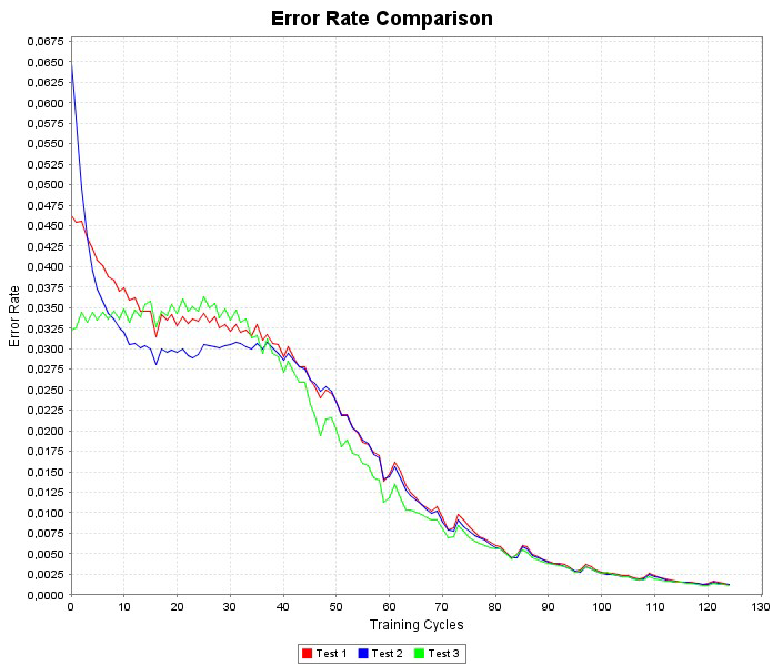
\includegraphics[width=0.7\columnwidth]{graphics/Error_time}
	\end{center}
	\vspace{-1em}
	\caption{A comparison using different initial weight values}
	\label{error_weights}
\vspace{1.5em}
\end{figure}

The result is that all calculated error rates differ in the first 100 training cycles. As it turns out after a training phase that is long enough all error rates conform the each other.
\pagebreak

\item [Number of hidden layers:] One feature that affects the time needed to train the neural network is the number of hidden layers. In this test the number of neurons in each hidden layer is set to the number of input nodes. Tests show that an increasing number of hidden layers raises the time needed to train the network but does not increase the quality of the resulting network.

Each test is performed with 10.000 training cycles. The result is shown in table \ref{train_layers} and figure \ref{error_hidden}. In addition to the amount of time needed, the number of training cycles to train the network also increases.

\begin{table}[htbp]
	\vspace{1.5em}
	\begin{center}
		\begin{tabular}{|l|l|l|}
		\hline
		\bf{Hidden layers}&\bf{Time needed}&{\bf Error rate}\\
		\hline
		1&5.658 sec&1.23151*$10^{-8}$\\
		\hline
		2&10.756 sec&2.13083*$10^{-8}$\\
		\hline
		3&15.602 sec&1.65828*$10^{-8}$\\
		\hline
		4&20.459 sec&3.89512*$10^{-8}$\\
		\hline
		\end{tabular}
	\end{center}
	\vspace{-1em}
	\caption{Resulting time and error when using 1, 2, 3 and 4 hidden layers}
	\label{train_layers}
\end{table}

\begin{figure}[htbp]
	\begin{center}
		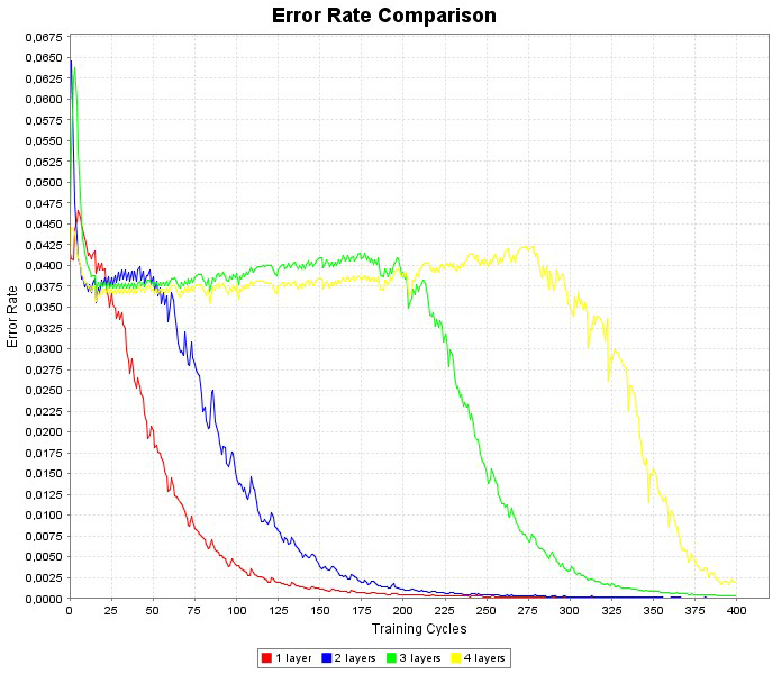
\includegraphics[width=0.7\columnwidth]{graphics/Error_hidden_layers}
	\end{center}
	\vspace{-1em}
	\caption{A comparison using 1, 2, 3 and 4 hidden layers}
	\label{error_hidden}
	\vspace{1.5em}
\end{figure}

Since the resulting error rate is not affected and the time needed to train the network increases with every additional layer the WIDS uses one hidden layer.

\pagebreak

	\item [Number of neurons in the hidden layers:] Table \ref{train_neurons} shows that choosing a higher number of neurons in a hidden layer can improve the resulting output of the network. On the other hand each additional neuron increases the time needed. Each test is performed with 10.000 training cycles.

\begin{table}[htbp]
	\vspace{1.5em}
	\begin{center}
		\begin{tabular}{|l|l|l|}
		\hline
		\bf{Neurons}&\bf{Time needed}&{\bf Error rate}\\
		\hline
		9&5.779 sec&2.09958*$10^{-8}$\\
		\hline
		18&9.263 sec&3.2259*$10^{-9}$\\
		\hline
		36&15.953 sec&2.23715*$10^{-9}$\\
		\hline
		72&30.634 sec&7.80079*$10^{-10}$\\
		\hline
		\end{tabular}
	\end{center}
	\vspace{-1em}
	\caption{Time needed to train the network using 9, 18, 36 and 72 neurons}
	\label{train_neurons}
\end{table}

Another test shows that it takes 30 seconds to test the neural network with 50000 packets and 18 hidden neurons. Therefore the WIDS can process 1666 packets per second. Assuming a 16 MBit WLAN and an average packet size of 1500 bytes it would be necessary to process 1333 packets per second in case the network operates at full capacity. That shows that the WIDS is fast enough to be used in a 16 MBit WLAN.

Due to the amount of time needed to train the network and the resulting performance of the test the WIDS uses 18 neurons in the hidden layer.

\vspace{1.5em}

	\item [Learning rate:] \cite{nn_learning_rate} states that "the larger the learning rate ... the larger the weight changes on each epoch, and the quicker the network learns. However, the size of the learning rate can also influence whether the network achieves a stable solution. If the learning rate gets too large, then the weight changes no longer approximate a gradient descent procedure". That means in other words that choosing a good learning rate results in better network performance than just setting it to a high value near $1$.

Figure \ref{error_learning_rates} shows the first 250 training cycles of the WIDS using different learning rates.

\begin{figure}[htbp]
	\begin{center}
		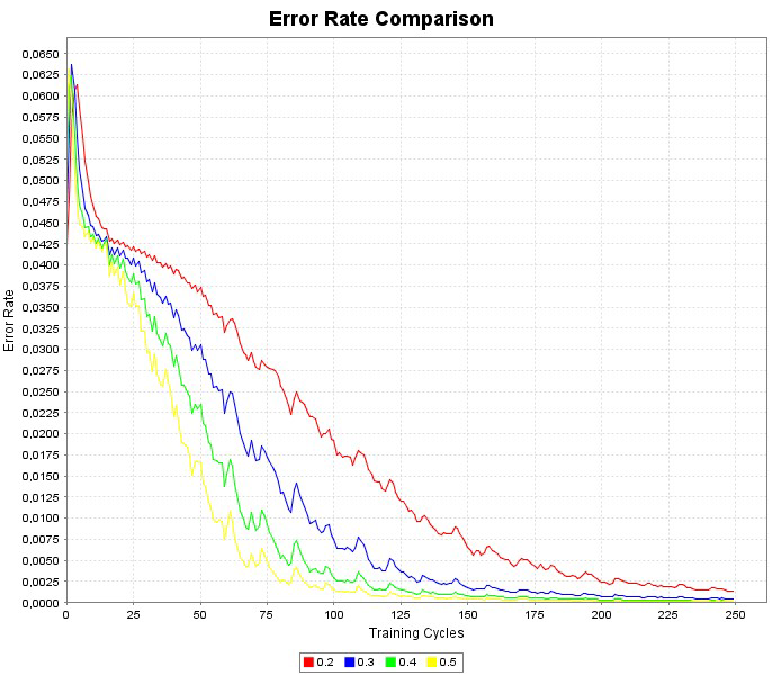
\includegraphics[width=0.7\columnwidth]{graphics/Error_learning_rates}
	\end{center}
	\vspace{-1em}
	\caption{A comparison using 0.2, 0.3, 0.4 and 0.5 as learning rate}
	\label{error_learning_rates}
\end{figure}

On the basis of these results and the warning not to choose a value that is too high the learning rate of the WIDS is set to $0.5$.

\vspace{1.5em}

	\item [Appearance of the sigmoid function:] As shown in figure \ref{error_sigmoid} the value for $a$ in the formula shown in section \ref{sec:activation} provides continuity for the learning process. The result of this test shows that the lower the value $a$ the smaller the difference between two steps in time is. In addition to that, the time needed to train a network increases.

\begin{figure}[htbp]
	\begin{center}
		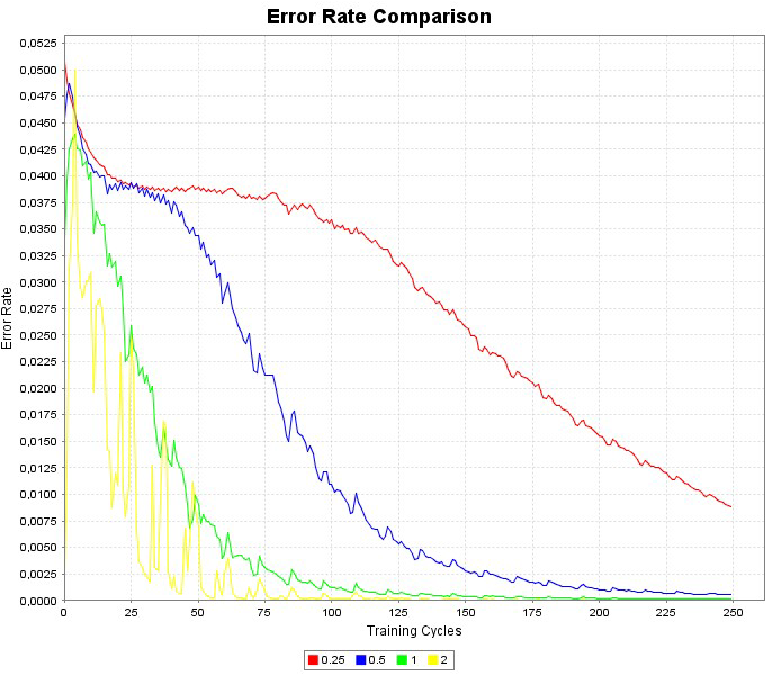
\includegraphics[width=0.7\columnwidth]{graphics/Error_sigmoid}
	\end{center}
	\vspace{-1em}
	\caption{A comparison using 0.25, 0.5, 1 and 2 for the sigmoid function}
\vspace{1.5em}
	\label{error_sigmoid}
\end{figure}

Since one single packet should not affect the obtained result too much and 
in order to avoid a learning process which takes a lot of time the WIDS uses the value of $1$ for $a$.

\end{description}

\section{WIDS}
\label{sec:results_wids}

The following section shows the results obtained by the WIDS. It uses a neural network with the configuration parameters shown in the previous section.

\subsection{Training}

The WIDS is trained by using previously stored pcap files. The characteristics of these files are shown in table \ref{train_env}.

The file in the {\em Normal traffic} column specifies the capture in which no attack occurs. It is a capture of the traffic in a WLAN which is WPA protected. It is created by using a WLAN NIC which is put into monitor mode and the tool Ethereal\footnote{Ethereal is a freely available packet capturing tool. It can be downloaded from http://www.ethereal.com/}.

\begin{table}[htbp]
	\begin{center}
		\begin{tabular}{|l|p{60pt}|p{60pt}|p{75pt}|}
		\hline
		&\bf{Normal traffic}&\bf{Association flood}&\bf{Disassociation flood} \\
		\hline
		Size&9738 KB&21 KB&20 KB\\
		\hline
		Time period&57 sec&9 sec&9 sec\\
		\hline
		Packet count&50000&500&500\\
		\hline
		Associations&5&500&0\\
		\hline
		Disassociations&4&0&500\\
		\hline
		\hline
		Rogue APs&0&0&0\\
		\hline
		Unknown clients&0&500&0\\
		\hline
		Association flood&no&yes&no\\
		\hline
		Disassociation flood&no&no&yes\\
		\hline
		\end{tabular}
	\end{center}
	\vspace{-1em}
	\caption{Properties of the files used for training the WIDS}
	\label{train_env}
\end{table}

The flood files specified in the {\em Association flood} and {\em Disassociation flood} column are created by using a self-made tool\footnote{This tool is named {\em DumpCreator} and is available on the shipped CD}. Both files consist of packets which are used for the respective flood attack only. The association flood uses random source addresses whereas the disassociation flood contains only those MACs as source which are also available in the respective WLAN where the WIDS is used.

\subsection{Testing}

After the training phase is finished the WIDS is tested. Table \ref{result_train} shows the average error values obtained when testing the network with the files used for training shown in table \ref{train_env}.

\begin{table}[htbp]
	\vspace{1.5em}
	\begin{center}
		\begin{tabular}{|l|p{60pt}|p{60pt}|p{75pt}|}
		\hline
		&\bf{Normal traffic}&\bf{Association flood}&\bf{Disassociation flood} \\
		\hline
		No attack&0.999285&0.0158409&0.00934418\\
		\hline
		Association flood&0.000839386&0.981713&0.00531103\\
		\hline
		Disassociation flood&0.00019222&0.00483618&0.988265\\
		\hline
		\hline
		Rogue APs&0&0&0\\
		\hline
		Unknown clients&0&500&0\\
		\hline
		\end{tabular}
	\end{center}
	\vspace{-1em}
	\caption{Average resulting error values using the training files}
	\vspace{1em}
	\label{result_train}
\end{table}

The WIDS identifies normal traffic with almost a 100\% certainty. The different flood attacks are identified with a guarantee of 98\%. Additionally, it detects 500 unknown clients when testing the association flood file since the client's source addresses were created randomly in this file.

The next test is performed with pcap files with the characteristics shown in table \ref{test_env}.

\begin{table}[htbp]
	\begin{center}
		\begin{tabular}{|l|l|l|l|l|}
		\hline
		&\bf{Test 1}&\bf{Test 2}&\bf{Test 3}&\bf{Test 4} \\
		\hline
		Size&9898 KB&10797 KB&10797 KB&10795 KB\\
		\hline
		Time period&65 sec&45 sec&45 sec&45 sec\\
		\hline
		Packet count&50000&50150&50150&50100\\
		\hline
		Associations&2&153&3&53\\
		\hline
		Disassociations&2&2&152&52\\
		\hline
		\hline
		Rogue APs&0&0&2&3\\
		\hline
		Unknown clients&0&149&0&49\\
		\hline
		Association flood&no&yes&no&yes\\
		\hline
		Disassociation flood&no&no&yes&yes\\
		\hline
		\end{tabular}
	\end{center}
	\vspace{-1em}
	\caption{Properties of the files used for testing the WIDS}
	\label{test_env}
\end{table}

The first test file is a capture of the WLAN with similar properties like the file used for training.

The second file is another capture of the WLAN but it also includes MACs of unknown clients and an association flood attack. The flood is performed using 149 association requests of clients with a randomised MAC address.

The third file includes two rogue APs and a disassociation flood. The flood is done by using 150 disassociation requests of legitimate clients.

The last test file contains all types of attacks. It uses 49 association requests and 50 disassociations of legitimate clients. Additionally, it contains 3 rogue APs and 49 unknown MAC addresses.

Table \ref{result_test} shows the results obtained when testing the WIDS using the files shown in table \ref{test_env}. The values in the rows named {\em Association floods} and {\em Disassociation floods} specify the number of feature sets\footnote{One feature set consists of all features described in section \ref{sec:features} and is created for every single packet received.} recognised that identify a specific attack. That means in other words that $0$ indicates that no attack occurs. All values above $0$ mean that one or more feature sets are found which characterise a certain flood attack.

\begin{table}[htbp]
	\vspace{1.5em}
	\begin{center}
		\begin{tabular}{|l|l|l|l|l|}
		\hline
		&\bf{Test 1}&\bf{Test 2}&\bf{Test 3}&\bf{Test 4} \\
		\hline
		Rogue APs&0&0&2&3\\
		\hline
		Unknown clients&0&149&0&49\\
		\hline
		Association floods&0&148&0&48\\
		\hline
		Disassociation floods&0&0&148&48\\
		\hline
		\end{tabular}
	\end{center}
	\vspace{-1em}
	\caption{The resulting numbers of attacks found in the test files}
	\label{result_test}
\end{table}

The test result of the first test file shows the desired result. No malicious activity is found.

In the second test file the WIDS finds the correct number of unknown clients and also detects an association flood. An interesting thing about this result is that the number of feature sets found that identify a flood attack is 148 and not 149. The reason is that the first packet of the flood attack is considered as normal traffic since the number of association packets in the past two seconds is still $0$. This shows that the WIDS alerts a flood attack in case the number of association packets received in a two second time slot exceeds $1$.

The results of the third test files show that the WIDS detects a disassociation flood attack in case the number of disassociations of legitimate clients in the past two seconds exceeds the value $2$. Again, the reason is that the first two disassociations of the attack are considered as valid. In addition to the flood attack both rogue APs are detected correctly.

The result of the fourth test file shows that the WIDS detects all attacks that occur in the network.

\chapter{Conclusion}

\section{Neural Networks for Intrusion Detection}

The results shown in section \ref{sec:results_wids} indicate that a neural network can be used efficiently in an intrusion detection system. A big advantage of using a neural network lies in the fact that the IDS can react to changes in the network characteristics.

Another important aspect is the preciseness of the system. If the characteristics in a WLAN do not change over time and the attacks are performed with enough packets the IDS detects all occurring association and disassociation flood attacks as well as malicious clients and rogue APs.

On the other hand there exist some drawbacks that an IDS developer needs to think of: Due to the complex structure of the neural network it is necessary to provide enough memory and computing power. Especially the training phase takes a lot of time depending on the amount of available data. Additionally, the network links between the data gatherer(s) and the data processor need to be faster than the speed in the WLAN network itself.

\section{Neural Networks and Traditional Methods}

\cite{nn_vs_traditional} poses the question whether it is better to use neural networks or traditional techniques\footnote{Traditional techniques in this context mean an anomaly based IDS which does not use a neural network. See section \ref{sec:sig_anom_ids} for details} to solve certain problems. The answer is that this is "an unanswerable question" \cite[p.4]{nn_vs_traditional}. The main problem lies in the characteristics of ANNs:

First, the weight values that are used to setup an uninitialised network are chosen randomly. This means the obtained results differ slightly each time the network is trained even if the same training set is used.

Next, as described in section \ref{sec:features}, the success of learning something is highly dependent on the features chosen for the input nodes. As a consequence the quality of the results differs significantly if different features are chosen.

Finally, the architecture and properties of the neural network itself change the results obtained. Section \ref{sec:test_nn} shows that depending on the number of hidden layers and neurons the performance of the network varies.

\section{Future Work}

The following section discusses tasks that need to be done before using the WIDS and possible improvements which make the WIDS more powerful.

\subsection{Putting the WIDS into a Real Network}

All tests have been done by using previously stored pcap files. The next step, to improve the WIDS, is to train it and put it in a WLAN to find out whether it behaves correctly and whether it reacts to changes in the network behaviour. This can only be done by running the WIDS over periods of several weeks and months.

Additionally, it is important to find out whether the neural network is fast enough to process the incoming traffic in real time or whether it is necessary to preprocess the traffic. In case the amount of traffic is too large for the neural network to handle it would be interesting to know how fast the WLAN may be until the WIDS can not process the data any longer.

\subsection{Adding Remote Functionality}

As described in section \ref{sec:design_wids} the design of the WIDS makes it possible to create remote sensors which collect data in a WLAN and send it to the data processor. As a consequence the data gathering component needs to be realised as a stand alone tool which connects to the data processor: The data processor is the server which waits for incoming data packets. Currently the WIDS does not support this form of client/server architecture.

\subsection{Adding Silent User Detection}

If a malicious user is present in a network but not sending any packets, it is impossible for the WIDS to detect this client because it needs packets to work with. As a consequence it is necessary to extend the WIDS with the capability to send RTS packets. As described in section \ref{sec:hidden_node_problem} the RTS/CTS handshake is used to overcome the hidden node problem. The answer to the RTS packet, the CTS frame, is sent automatically. This means that it is not possible (at least with unmodified hardware) to prevent the sending of a CTS packet. The RTS/CTS handshake makes it possible to detect clients although they do not send packets.

A drawback of this method is that a client needs to be known as malicious because it is necessary to know the MAC address to which the RTS packet is sent to.

\subsection{Adding Scanner Fingerprinting}

As described in \cite{wlan_fingerprints} some active wireless scanners like Netstumbler or Wellenreiter provide individual characteristics when they send frames. That makes it possible to find out what type of scanner an intruder is using.

\subsection{Reacting on Intrusions}

Currently the WIDS writes an alert message on the screen whenever a flood attack is recognised or an unknown MAC address is found. The next step is to react to possible threats automatically. Possible counter measures include modifying the firewall to block a certain client or to send a mail to the network administrator to inform about ongoing threats.

\subsection{Providing a GUI}

Currently the WIDS alerts the user by printing a message on the screen. It would be easier to configure and handle this tool if it is based on a GUI. It could consist of a configuration section which is capable of changing the structure of the neural network. Additionally, it should be possible to perform the training and testing phase of the WIDS graphically.

\section{Outlook}

As explained in \cite{IDS_terminology} "Intrusion Detection Systems (IDS) are still in their infancy" and as a consequence used very rarely. On the other hand it is a very fast evolving area in computer science.

The underlying work shows that using a neural network can be advantageous and will very likely find its way in upcoming (wireless) intrusion detection systems.


% Create an Appendix
\input{Appendix}

% Create a list of figures
\listoffigures
% Create a list of tables
\listoftables
% Create a glossary
\printglosstex(acr)

% Set bibliography style
\bibliographystyle{apalike}
% Create a bibliography
\bibliography{Bibliography}

\end{document}

